%!TEX root = presentation.tex

\subsection{Introduction}

\begin{frame}{Outline}
    Situation calculus provides a framework for reasoning about actions.

    This work presents an expansion to handle the \textit{knowledge} possessed or acquired by the agent,
    and allow it to shape the agent's decisions.
    \begin{itemize}%[<+->]
        \item Knowledge is represented by one additional fluent
        \item Uniform axiomatization with the rest of sitcalc
        \item Ordinary actions and knowledge-producing ones are strictly separated
        \item Easy expansion of regression as defined in [Reiter2001]
        \item Desirable properties are direct consequences of the axiomatization \\
                (e.g. knowledge persistence / memory)
    \end{itemize}
\end{frame}

% opzionale
\begin{frame}{...}
    Opzionale

    Un paio di azioni ordinarie e un paio di azioni di conoscenza di esempio, giusto per inquadrare il discorso
\end{frame}

\subsection{Knowledge as a fluent}

\begin{frame}[fragile]{The K fluent}
    \huge
    \[ \textfluent{K}(s', s) \]
    \normalsize

    Defines an accessibility relation between situations.

    % Informal definition: \( \textfluent{K}(s', s) \) is true if, given its current knowledge,
    % the situations \(s\) and \(s'\) are indistinguishable to the agent.

    \begin{block}{(Informal) definition}
        \( \textfluent{K}(s',s) \) is true if an agent in situation \(s\)
        could mistake the current situation for the other \(s'\),
        given its current knowledge.
    \end{block}
\end{frame}

\begin{frame}{Knowledge}
    \begin{block}{Definition of knowledge}
        A fluent is known to be true (false) in a situation \(s\)
        if and only if it is true (false)
        in all situations accessible from \(s\).
    \end{block}

    Shorthand notation: \( \knows(\phi, s) \defeq \forall s' \: \textfluent{K}(s',s) \rightarrow \phi(s') \)
\end{frame}

\begin{frame}{Knowledge-producing actions}
    Actions that have an effect on the agent's knowledge

    \begin{block}{SENSE actions}
        % Learn whether a fluent is true or false. Example: check if a door is open or closed.
        Learn the truth value of a formula. Example: check if a door is open or closed.
        \[
            \knows(\textfluent{P}, \textfluent{DO}(\textfluent{SENSE}_\text{P}, s))
            \lor
            \knows(\lnot \textfluent{P}, \textfluent{DO}(\textfluent{SENSE}_\text{P}, s))
        \]
    \end{block}

    \begin{block}{READ actions}
        % Learn what a functional term refers to. Example: read a number on a sheet of paper.
        Learn the value of a term. Example: read a number on a sheet of paper.
        \[
            \exists x \: \knows(\tau = x, \textfluent{DO}(\textfluent{READ}_\tau, s))
        \]
    \end{block}

    \emph{Assumption: ordinary and knowledge-producing actions are strictly separated.}
\end{frame}

\subsection{Knowledge effects}

\begin{frame}{Towards a successor state axiom for K}
    In order to complete the specification of the \textfluent{K} fluent,
    we need to define its successor state axiom,
    determining how ordinary actions and knowledge-producing actions affect it.

    Consider this case study with three accessible situations. The agent is in S1.

    \begin{center}
        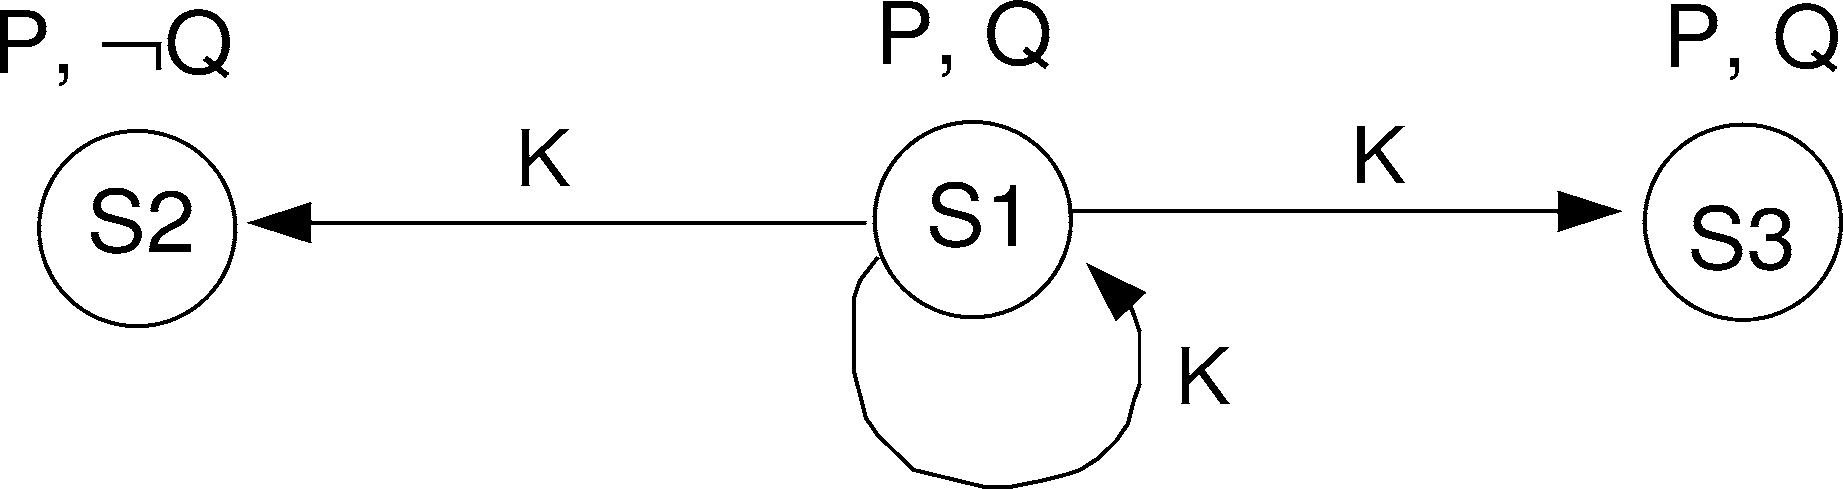
\includegraphics[width=0.6\textwidth]{assets/3states_noactions.png}
    \end{center}

    \[ \knows(\textfluent{P}, S1) \land \lnot \knows(\textfluent{Q}, S1) \]
\end{frame}

\begin{frame}{Ordinary actions}
    Pippo
\end{frame}

\begin{frame}{Knowledge-producing actions}
    Pippo
\end{frame}

\begin{frame}{The successor state axiom for K}
    Pippo
\end{frame}

\begin{frame}{<varie ed eventuali>}
    Pippo
\end{frame}
